\chapter{Maximal extension of Schwarzschild spacetime}
\label{s:max}

\minitoc

\section{Introduction}


%%%%%%%%%%%%%%%%%%%%%%%%%%%%%%%%%%%%%%%%%%%%%%%%%%%%%%%%%%%%%%%%%%%%%%%%%%%%%%%


\section{Kruskal-Szekeres coordinates}

\subsection{Definition} \label{s:sch:KS_coord}

On the open set $\M_{\rm I}$, let us consider the ``double-null''
coordinate system $\hat{\hat{x}}^\alpha = (u,v,\th,\ph)$. It is related to
Schwarzschild-Droste coordinates $(t,r,\th,\ph)$ by
Eqs.~(\ref{e:sch:outgoing_null_geod})-(\ref{e:sch:ingoing_null_geod}):
\be \label{e:sch:u_v_r_t}
    \left\{\begin{array}{l}
    u = t - r - 2 m \ln \left| \frac{r}{2m} - 1 \right| \\[1ex]
    v = t + r + 2 m \ln \left| \frac{r}{2m} - 1 \right|
    \end{array}\right.
    \iff
        \left\{\begin{array}{l}
    t = \frac{1}{2} (u+v)\\[1ex]
    r + 2 m \ln \left| \frac{r}{2m} - 1 \right| = \frac{1}{2} (v-u).
    \end{array}\right.
\ee
Despite one cannot express explicitely $r$ in terms of $(u,v)$,
the function $r\mapsto r + 2 m \ln \left| \frac{r}{2m} - 1 \right|$ is
invertible on $(2m,+\infty)$ (cf. Fig.~\ref{f:sch:tortoise}), so that (\ref{e:sch:u_v_r_t}) does define a coordinate system on $\M_{\rm I}$.
The range of $(u,v)$ is $\R^2$.

The above relations imply
\[
 \D u = \D t - \frac{\D r}{1 - \frac{2m}{r}}  \qquad\mbox{and}\qquad
\D v = \D t + \frac{\D r}{1 - \frac{2m}{r}} .
\]
Hence
\[
    \D u \, \D v = \D t^2 - \frac{\D r^2}{\left(1 - \frac{2m}{r} \right) ^2} .
\]
The line element (\ref{e:sch:Schwarz_metric_SD}) becomes then
\be \label{e:sch:Schwarz_metric_uv}
    \encadre{
        \hat{\hat{g}}_{\mu\nu}\, \D \hat{\hat{x}}^\mu \,
        \D \hat{\hat{x}}^\nu =
            -\left( 1 - \frac{2 m}{r} \right)\, \D u \, \D v
       +  r^2 \left( \D\th^2 + \sin^2\th\, \D\ph^2 \right) }.
\ee
In this formula, $r$ is to be considered as a function of $(u,v)$, given
by (\ref{e:sch:u_v_r_t}).

\begin{figure}
\centerline{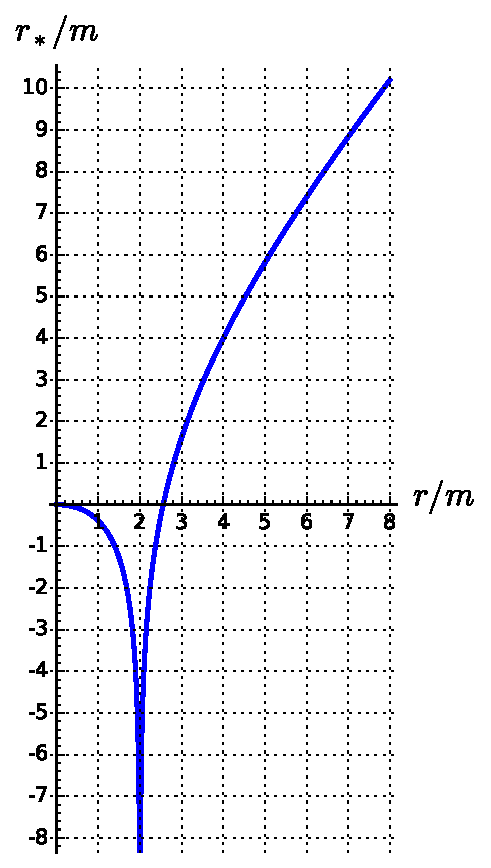
\includegraphics[height=0.4\textheight]{sch_tortoise.pdf}}
\caption[]{\label{f:sch:tortoise} \footnotesize
Function $r_*(r) = r + 2 m \ln \left| \frac{r}{2m} - 1 \right|$
(the tortoise coordinate, cf. Eq.~(\ref{e:sch:def_tortoise})).
It relates $r$ to $(u,v)$ via $r_*(r) = (u-v)/2$ [Eq.~(\ref{e:sch:u_v_r_t})].}
\end{figure}

The metric components (\ref{e:sch:Schwarz_metric_uv}) are regular on $\M_{\rm I}$.
Having a look at Fig.~\ref{f:sch:tortoise}, we realize that we cannot extend
this coordinate system to include the Schwarzschild horizon $\Hor$, since
$r\rightarrow 2m$ is equivalent to $v-u\rightarrow -\infty$: if $u$ (resp. $v$)
were taking a finite value on $\Hor$, we would have $v\rightarrow -\infty$
(resp. $u\rightarrow +\infty$). This impossibility of extending to $\Hor$
is also reflected by the fact that
\[
    \det \left( \hat{\hat{g}}_{\alpha\beta} \right) =
        - \frac{1}{4} \left( 1 - \frac{2 m}{r} \right) ^2 r^4 \sin^2\th
\]
vanishes for $r\rightarrow 2m$, which would make $\w{g}$ a degenerate bilinear
form at $r=2m$, while it is not of course.

Instead of $(u,v)$, let us use on $\M_{\rm I}$
the coordinates $(U,V)$ defined by
\be \label{e:sch:def_U_V}
    \left\{\begin{array}{l}
    U := - \mathrm{e}^{-u/4m} \\
    V := \mathrm{e}^{v/4m} .
    \end{array}\right.
\ee
Since the range of $(u,v)$ is $\R^2$, the range of $U$ is $(-\infty,0)$
and that of $V$ is $(0,+\infty)$.
We have
\[
    \D U = \frac{1}{4m} \,  \mathrm{e}^{-u/4m}  \, \D u\qquad\mbox{and}\qquad
    \D V = \frac{1}{4m} \,  \mathrm{e}^{v/4m} \, \D v ,
\]
hence
\[
    \D u \, \D v = 16 m^2 \mathrm{e}^{(u-v)/4m} \, \D U \, \D V .
\]
Now, on $\M_{\rm I}$, $r>2m$ and (\ref{e:sch:u_v_r_t}) yields
\be \label{e:sch:r_u_v_exp}
    r + 2 m \ln \left( \frac{r}{2m} - 1 \right) = \frac{1}{2} (v-u)
    \quad
    \Longrightarrow
    \quad
     \mathrm{e}^{r/2m} \left( \frac{r}{2m} - 1 \right)  =
    \mathrm{e}^{(v-u)/4m}  ,
\ee
so that
\[
     \D u \, \D v = 16 m^2 \, \mathrm{e}^{-r/2m}
        \left( \frac{r}{2m} - 1 \right) ^{-1} \D U \, \D V
        = \frac{32 m^3}{r} \, \mathrm{e}^{-r/2m}
        \left( 1 - \frac{2m}{r} \right) ^{-1} \D U \, \D V .
\]
Substituting this expression in (\ref{e:sch:Schwarz_metric_uv}) yields
the expression of the metric components with respect to
coordinates ${\hat X}^\alpha := (U,V,\th,\ph)$:
\be \label{e:sch:metric_UV}
    \encadre{
    g_{\mu\nu} \, \D {\hat X}^\mu \, \D {\hat X}^\nu =
    - \frac{32 m^3}{r} \, \mathrm{e}^{-r/2m} \,  \D U \, \D V
     +  r^2 \left( \D\th^2 + \sin^2\th\, \D\ph^2 \right) }.
\ee
In this formula, $r$ has to be considered as a function of $(U,V)$, whose
implicit expression is found by combining
(\ref{e:sch:def_U_V}) and (\ref{e:sch:r_u_v_exp}):
\be \label{e:sch:r_UV}
    \encadre{ \mathrm{e}^{r/2m} \left( \frac{r}{2m} - 1 \right) = - U V } .
\ee
\begin{remark}
This relation takes a very simple form in terms of the tortoise coordinate
(cf. Eq.~(\ref{e:sch:def_tortoise})):
\[
    \mathrm{e}^{r_*/2m} = - U V  .
\]
\end{remark}

We notice that the factor $(1-2m/r)$ has disappeared in the line
element (\ref{e:sch:metric_UV}), which becomes perfectly regular as
$r\rightarrow 2m$.

We read on (\ref{e:sch:metric_UV}) that $g_{UU} = 0$ and $g_{VV} = 0$.
Hence $(U,V)$ is a double-null coordinate system, as much as $(u,v)$.
To cope with a timelike-spacelike coordinate system instead, let
us introduce on $\M_{\rm I}$ the pair $(T,X)$ such that $U$ is $T$
retarded by $X$ and $V$ is $T$ advanced by $X$:
\be \label{e:sch:def_T_X}
    \left\{\begin{array}{l}
    U = T - X\\
    V = T + X
    \end{array}\right.
    \qquad \iff\qquad
    \left\{\begin{array}{l}
    T = \frac{1}{2} (U+V) \\[1ex]
    X = \frac{1}{2} (V-U)
    \end{array}\right.
\ee
Since the range of $U$ on $\M_{\rm I}$ is $(-\infty,0)$ and that of $V$ is
$(0,+\infty)$, the range of $(T,X)$ is ruled by $T<X$, $T>-X$ and $X>0$.
In other words, the coordinates $(T,X)$ span the following quarter of
$\mathbb{R}^2$ (cf. Fig.~\ref{f:sch:SD_I_KS}):
\be \label{e:sch:X_T_range_I}
    \M_{\rm I}: \quad X > 0 \quad\mbox{and}\quad -X < T < X .
\ee
The coordinates $X^\alpha := (T,X,\th,\ph)$ are called
the \defin{Kruskal-Szekeres coordinates}\index{Kruskal-Szekeres!coordinates}.

\begin{figure}
\centerline{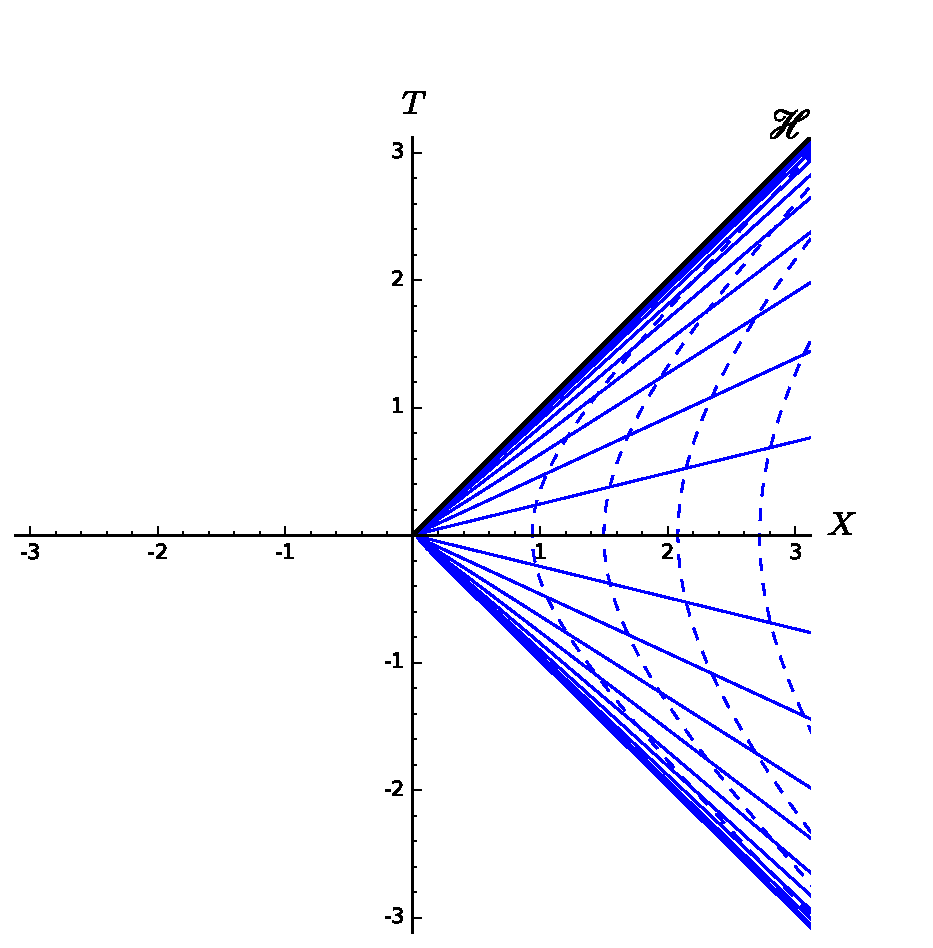
\includegraphics[width=0.6\textwidth]{sch_SD_I_KS.pdf}}
\caption[]{\label{f:sch:SD_I_KS} \footnotesize
Submanifold $\M_{\rm I}$ in the Kruskal-Szekeres coordinates $(T,X)$:
$\M_{\rm I}$ is covered by the Schwarzschild-Droste grid (in blue): the solid
lines have $t=\mathrm{const}$ (spaced apart by $\delta t = m$), while the
dashed curves have $r=\mathrm{const}$ (spaced apart by $\delta r = m/2$).}
\end{figure}


We have $\D U \, \D V = (\D T - \D X) (\D T + \D X)  = \D T^2 - \D X^2$,
so that the metric components with respect to the Kruskal-Szekeres coordinates
are easily deduced from the line element (\ref{e:sch:metric_UV}):
\be \label{e:sch:metric_KS}
    \encadre{
    g_{\mu\nu} \, \D X^\mu \, \D X^\nu =
    \frac{32 m^3}{r} \, \mathrm{e}^{-r/2m}
    \left( - \D T^2 + \D X^2 \right)
     +  r^2 \left( \D\th^2 + \sin^2\th\, \D\ph^2 \right) }.
\ee
Here $r$ is to be considered as the function of $(T,X)$ that is defined
implicitely by
\be \label{e:sch:X2mT2}
   \encadre{ \mathrm{e}^{r/2m} \left( \frac{r}{2m} - 1 \right) = X^2 - T^2 } .
\ee
This relation is a direct consequence of (\ref{e:sch:r_UV}) and (\ref{e:sch:def_T_X}).
We may rewrite it as
\be
    \mathrm{e}\, f\left( \frac{r}{2m} - 1 \right) = X^2 - T^2,
\ee
where $f$ is the function defined by
\be \label{e:sch:def_F}
    \begin{array}{cccc}
    f: & (-1,+\infty) & \longrightarrow & (-1/\mathrm{e},+\infty) \\
        & x & \longmapsto & x \mathrm{e}^{x} .
    \end{array}
\ee
The graph of $f$  is shown in Fig.~\ref{f:max:xex}. We see clearly that it is a bijective map.
In particular, $F$ induces a bijection between $(1,+\infty)$ (the range of $r/2m$ on $\M_{\rm I}$)
and $(0,+\infty)$ (the range of $X^2-T^2$ on $\M_{\rm I}$, according to (\ref{e:sch:X_T_range_I})).
Hence, in the line element (\ref{e:sch:metric_KS}), we may write
$r = 2m F^{-1}(X^2-T^2)$. Noticing that
$2m/r \, \mathrm{e}^{-r/2m} = (X^2-T^2 + \mathrm{e}^{r/2m})^{-1}$
[cf. Eq.~(\ref{e:sch:X2mT2})], we may eliminate $r$ from the expression
of the metric components in Kruskal-Szekeres coordinates:
\be \label{e:sch:metric_KS_TX_partial}
   \encadre{
    \begin{array}{lcll}
    g_{\mu\nu} \, \D X^\mu \, \D X^\nu & = & 4m^2 \bigg\{ & \displaystyle
    \frac{4}{X^2-T^2 + \mathrm{e}^{F^{-1}(X^2-T^2)} }
    \left( - \D T^2 + \D X^2 \right) \\[2ex]
    & & & \displaystyle + \,   (F^{-1}(X^2-T^2))^2 \left( \D\th^2 + \sin^2\th\, \D\ph^2 \right)
    \bigg\}.
    \end{array} }
\ee


\begin{figure}
\centerline{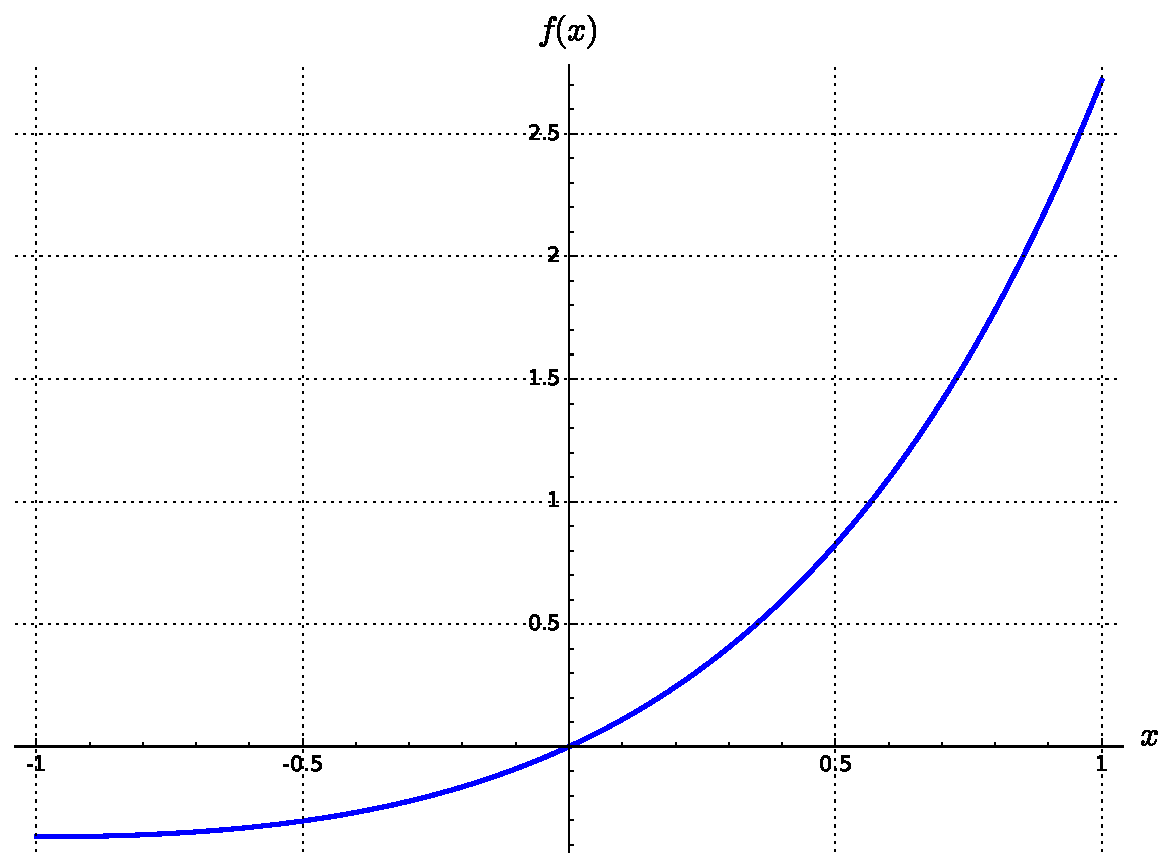
\includegraphics[height=0.37\textheight]{max_xex.pdf}}
\caption[]{\label{f:max:xex} \footnotesize
Function $f(x) = x \mathrm{e}^{x}$, giving
$X^2-T^2 = \mathrm{e} \, f(r/2m-1)$, cf. Eq.~(\ref{e:sch:X2mT2}).}
\end{figure}


The relation between the Kruskal-Szekeres coordinates and the
Schwarzschild-Droste ones is obtained by combining (\ref{e:sch:def_T_X}),
(\ref{e:sch:def_U_V}) and (\ref{e:sch:u_v_r_t}):
\bea
    T &=& \frac{1}{2}(U+V) = \frac{1}{2} \left( \mathrm{e}^{v/4m}
        - \mathrm{e}^{-u/4m)} \right) =
        \frac{1}{2} \left( \mathrm{e}^{(t+r_*)/4m}
        - \mathrm{e}^{(r_*-t)/4m} \right) \nonumber \\
     & = & \mathrm{e}^{r_*/4m} \sinh\left( \frac{t}{4m} \right) ,\nonumber
\eea
where $r_*$ is related to $r$ by (\ref{e:sch:def_tortoise}).
Similarly
\[
     X = \mathrm{e}^{r_*/4m} \cosh\left( \frac{t}{4m} \right) .
\]
In particular, we have
\[
    \frac{T}{X} = \tanh\left( \frac{t}{4m} \right) .
\]
From Eq.~(\ref{e:sch:def_tortoise}), we have
\[
    \mathrm{e}^{r_*/4m} = \mathrm{e}^{r/4m} \sqrt{ \frac{r}{2m} - 1 } .
\]
We may summarize the above relations as follows:
\be \label{e:sch:KS_SD_I}
    \M_{\rm I}: \quad \encadre{ \left\{\begin{array}{l}
    T = \mathrm{e}^{r/4m} \sqrt{ \frac{r}{2m} - 1 } \sinh\left( \frac{t}{4m} \right)
\\[2ex]
    X = \mathrm{e}^{r/4m} \sqrt{ \frac{r}{2m} - 1 } \cosh\left( \frac{t}{4m} \right)
        \end{array}\right. }
    \iff
    \encadre{ \left\{\begin{array}{l}
    t = 2 m \,  \ln \left( \frac{X+T}{X-T} \right) \\[2ex]
    r = 2 m F^{-1}(X^2 - T^2) .
        \end{array}\right. }
\ee
Note that we have used the identity $\mathrm{artanh}\, x = 1/2 \ln\left[(1+x)/(1-x)\right]$.
The curves of constant $t$ and constant $r$ in the $(T,X)$ plane
are drawn in Fig.~\ref{f:sch:SD_I_KS}.
\begin{remark}
Given the properties of the $\cosh$ and $\sinh$ functions, it is clear on these
expressions that the constraints (\ref{e:sch:X_T_range_I}) are satisfied.
\end{remark}
\begin{remark}
In line element (\ref{e:sch:metric_KS_TX_partial})
the metric components $g_{TT}$ and $g_{XX}$ depend on both $X$ and $T$; this
shows that neither $\wpar_T$ nor $\wpar_X$ coincide with a Killing vector.
In other words, the coordinates $(T,X)$ are not adapted to the spacetime
symmetries, contrary to the Schwarzschild-Droste coordinates or to the
Eddington-Finkelstein ones.
\end{remark}

\subsection{Extension to the IEF domain}

We notice that the metric components (\ref{e:sch:metric_KS}) are perfectly
regular at $r=2m$. Therefore the Kruskal-Szekeres coordinates can be extended
to cover the Schwarzschild horizon $\Hor$. Actually they can be extended to
all values of $r\in (0,2m]$, i.e. to the whole domain of the ingoing
Eddington-Finkelstein coordinates: the manifold $\M_{\rm IEF}$ introduced
in Sec.~\ref{s:sch:Schwarz_hor}:
$\M_{\rm IEF} = \M_{\rm I} \cup \Hor \cup \M_{\rm II}$. Let us show
this in detail. Back on $\M_{\rm I}$, we can express the IEF coordinate
$\ti$ in terms of $(T,X)$ by combining $\ti = v - r$ [Eq.~(\ref{e:sch:ti_v_r})],
$v = 4m\ln V$ [Eq.~(\ref{e:sch:def_U_V})] and $V = T+X$ [Eq.~(\ref{e:sch:def_T_X})]:
\be
    \ti = 4 m \ln (T+X) - r.
\ee
The above relation is a valid expression as long as $T+X>0$.
Besides, we already noticed
that the function $F$ defined by (\ref{e:sch:def_F}) is a bijection from the range of $r/2m$
on $\M_{\rm IEF}$, i.e. $(0,+\infty)$, to $(-1,+\infty)$, with the
$(0,+\infty)$ part of the latter interval representing the range of $X^2-T^2$
on $\M_{\rm I}$. We may use these properties to extend the Kruskal-Szekeres coordinates to all $\M_{\rm IEF}$ by requiring
\begin{subequations}
\label{e:sch:ti_r_X_T}
\begin{align}
 & \ti = 4 m \ln (T+X) - r\\
 & \underbrace{\mathrm{e}^{r/2m} \left( \frac{r}{2m} - 1 \right)}_{F(r/2m)} = X^2-T^2 .
 \end{align}
\end{subequations}
The range of the coordinates $(T,X)$ on $\M_{\rm IEF}$ is then ruled by
\[
    \M_{\rm IEF}:\quad T+X > 0 \quad\mbox{and}\quad X^2 - T^2 > -1 ,
\]
which can be rewritten as
\be \label{e:sch:range_X_T_IEF}
    \M_{\rm IEF}: \quad -X < T < \sqrt{X^2+1}.
\ee
We deduce from (\ref{e:sch:ti_r_X_T}) that
\be \label{e:sch:KS_IEF_prov}
    \left\{\begin{array}{lcl}
    X+T & = & \mathrm{e}^{(\ti+r)/4m} \\
    X-T & = & \mathrm{e}^{(r -\ti)/4m} \left( \frac{r}{2m} - 1 \right) .
    \end{array}\right.
\ee
Hence the relation between the ingoing Eddington-Finkelstein coordinates and
the Kruskal-Szekeres ones on $\M_{\rm IEF}$:
\be \label{e:sch:KS_IEF}
    \encadre{ \left\{\begin{array}{l}
    T = \mathrm{e}^{r/4m} \left[ \cosh\left(\frac{\ti}{4m}\right)
        - \frac{r}{4m} \mathrm{e}^{-\ti/4m} \right] \\[2ex]
    X =  \mathrm{e}^{r/4m} \left[ \sinh\left(\frac{\ti}{4m}\right)
        + \frac{r}{4m} \mathrm{e}^{-\ti/4m}  \right]
    \end{array}\right. }
    \iff
    \encadre{\left\{\begin{array}{l}
     \ti =  2 m \left[ 2 \ln (T+X) - F^{-1}(X^2 - T^2) \right] \\[1ex]
    r = 2 m F^{-1}(X^2 - T^2)
    \end{array}\right. }
\ee
The various subsets of $\M_{\rm IEF}$ correspond then to the following
coordinate ranges (cf. Fig.~\ref{f:sch:IEF_KS}):
\begin{subequations}
\begin{align}
 & \M_{\rm I}: \quad X > 0 \quad\mbox{and}\quad -X < T < X \\
 & \Hor: \quad X > 0 \quad\mbox{and}\quad  T = X \\
 & \M_{\rm II}: \quad |X| < T < \sqrt{X^2+1} .
\end{align}
\end{subequations}

\begin{figure}
\centerline{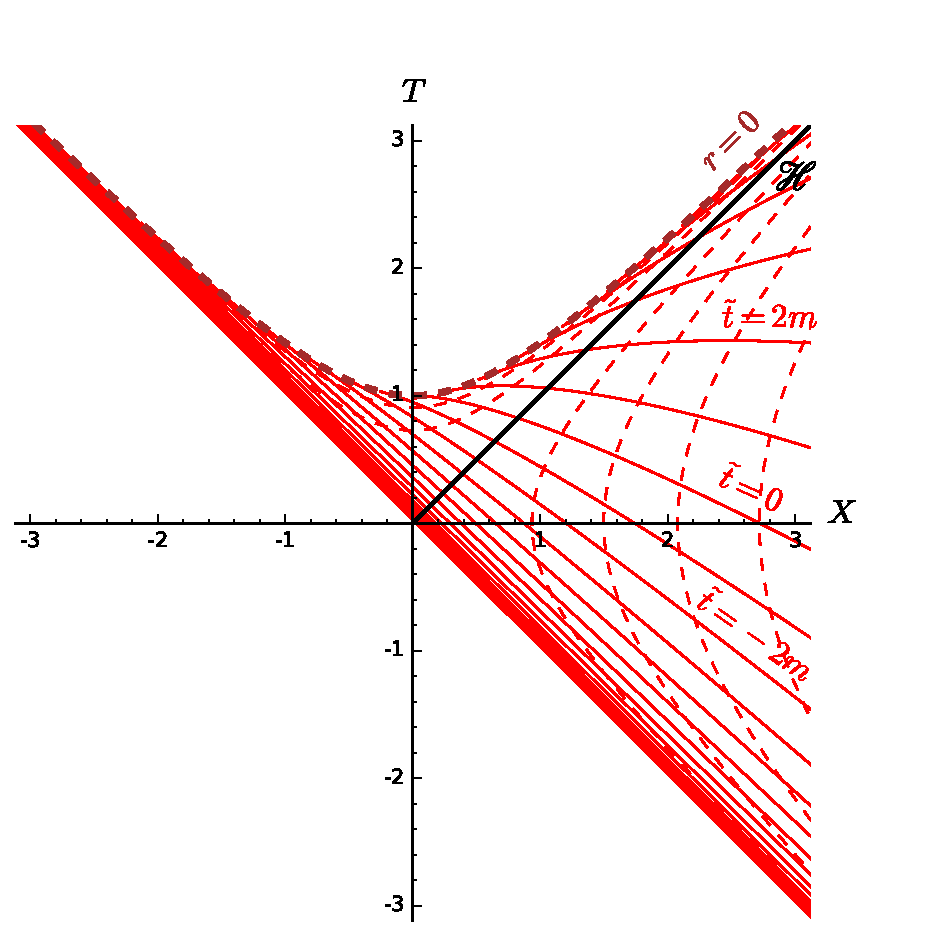
\includegraphics[width=0.6\textwidth]{sch_IEF_KS.pdf}}
\caption[]{\label{f:sch:IEF_KS} \footnotesize
Domain of ingoing Eddington-Finkelstein coordinates, $\M_{\rm IEF} = \M_{\rm I}\cup \Hor\cup \M_{\rm II}$, depicted in terms of the Kruskal-Szekeres coordinates $(T,X)$: the solid red
curves have $\ti=\mathrm{const}$ (spaced apart by $\delta\ti = m$), while the
dashed red curves have $r=\mathrm{const}$ (spaced apart by $\delta r = m/2$).}
\end{figure}


Since the relation between IEF coordinates and Kruskal-Szekeres ones is the
same in $\M_{\rm II}$ as in $\M_{\rm I}$ (being given by (\ref{e:sch:KS_IEF})
in both cases), we conclude that the expression (\ref{e:sch:metric_KS})
of the metric components with respect to
Kruskal-Szekeres coordinates is valid in all $\M_{\rm IEF}$.

Let us determine the relation between the Kruskal-Szekeres coordinates and
the Schwarz\-schild-Droste ones in $\M_{\rm II}$. Since $r<2m$ in $\M_{\rm II}$,
Eq.~(\ref{e:sch:ti_t_r}) gives
\[
    \M_{\rm II}: \quad  \mathrm{e}^{\ti/4m} = \mathrm{e}^{t/4m}  \sqrt{1 -  \frac{r}{2m} } ,
\]
so that (\ref{e:sch:KS_IEF_prov}) can be rewritten as
\[
     \M_{\rm II}: \quad
\left\{\begin{array}{lcl}
    X+T & = & \displaystyle \mathrm{e}^{(t+r)/4m} \sqrt{1 -  \frac{r}{2m} }  \\[2ex]
    X-T & = & \displaystyle  - \mathrm{e}^{(r -t)/4m}  \sqrt{1 -  \frac{r}{2m} }.
    \end{array}\right.
\]
We obtain then
\be \label{e:sch:KS_SD_II}
    \M_{\rm II}: \quad \encadre{ \left\{\begin{array}{l}
    T = \mathrm{e}^{r/4m} \sqrt{ 1 - \frac{r}{2m} } \cosh\left( \frac{t}{4m} \right)
\\[2ex]
    X = \mathrm{e}^{r/4m} \sqrt{ 1 - \frac{r}{2m} } \sinh\left( \frac{t}{4m} \right)
        \end{array}\right. }
    \iff
    \encadre{ \left\{\begin{array}{l}
    t = 2 m \,  \ln \left( \frac{T+X}{T-X} \right) \\[2ex]
    r = 2 m F^{-1}(X^2 - T^2) .
        \end{array}\right. }
\ee
This is to be compared with (\ref{e:sch:KS_SD_I}).
The curves of constant $t$ and constant $r$ in the $(T,X)$ plane
are drawn in Fig.~\ref{f:sch:SD_KS}, which extends Fig.~\ref{f:sch:SD_I_KS}
to $\M_{\rm II}$.

\begin{figure}
\centerline{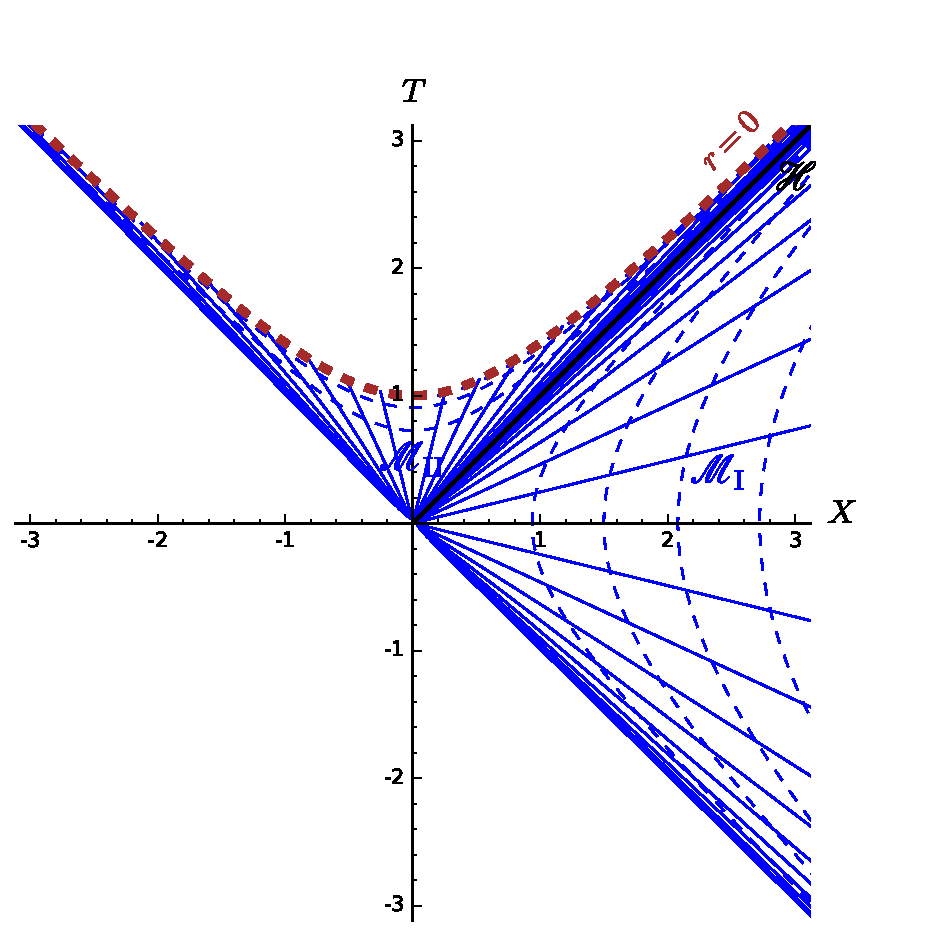
\includegraphics[width=0.6\textwidth]{sch_SD_KS.pdf}}
\caption[]{\label{f:sch:SD_KS} \footnotesize
Schwarzschild-Droste coordinates in $\M_{\rm SD} = \M_{\rm I}\cup \M_{\rm II}$
depicted in terms of the Kruskal-Szekeres coordinates $(T,X)$: the solid blue
curves have $t=\mathrm{const}$ (spaced apart by $\delta t = m$), while the
dashed blue curves have $r=\mathrm{const}$ (spaced apart by $\delta r = m/2$).}
\end{figure}


As discussed in Sec.~\ref{s:sch:singularities}, one approaches a
curvature singularity as $r\rightarrow 0$. According to (\ref{e:sch:KS_IEF})
or (\ref{e:sch:KS_SD_II}),
this corresponds to $X^2-T^2 \rightarrow -1$ (see also Fig.~\ref{f:sch:X2mT2}), with
$T > 0$. Hence, in the $(T,X)$ plane, the curvature singularity is located
at $T = \sqrt{X^2 + 1}$, i.e. at the upper branch of the hyperbola
$X^2 - T^2 = -1$.

\subsection{Radial null geodesics in Kruskal-Szekeres coordinates}
\label{s:sch:rad_null_geod_KS}

By construction, the Kruskal-Szekeres coordinates $(T,X,\th,\ph)$ are
adapted to the radial null geodesics. This is clear on the expression
(\ref{e:sch:metric_KS}) of the metric tensor, where the $(T,X)$ part is
conformal to the flat metric $- \D T^2 + \D X^2$. Consequently the radial
null geodesics are straight lines of slope $\pm 45^\circ$ in the $(T,X)$ plane
(cf. Fig.~\ref{f:sch:rad_null_geod_KS}):
\begin{itemize}
\item the ingoing radial null geodesics obey
\be
    T = - X + V ,
\ee
where $V$ is a positive constant (the constraint $V>0$ following from (\ref{e:sch:range_X_T_IEF})), so that each geodesic of this family can be labelled
by $(V,\th,\ph)$;
\item the outgoing radial null geodesics obey
\be \label{e:sch:outgoing_null_geod_KS}
    T = X + U ,
\ee
where $U$ is an arbitrary real constant, so that each geodesic of this family can be labelled
by $(U,\th,\ph)$.
\end{itemize}
\begin{figure}
\centerline{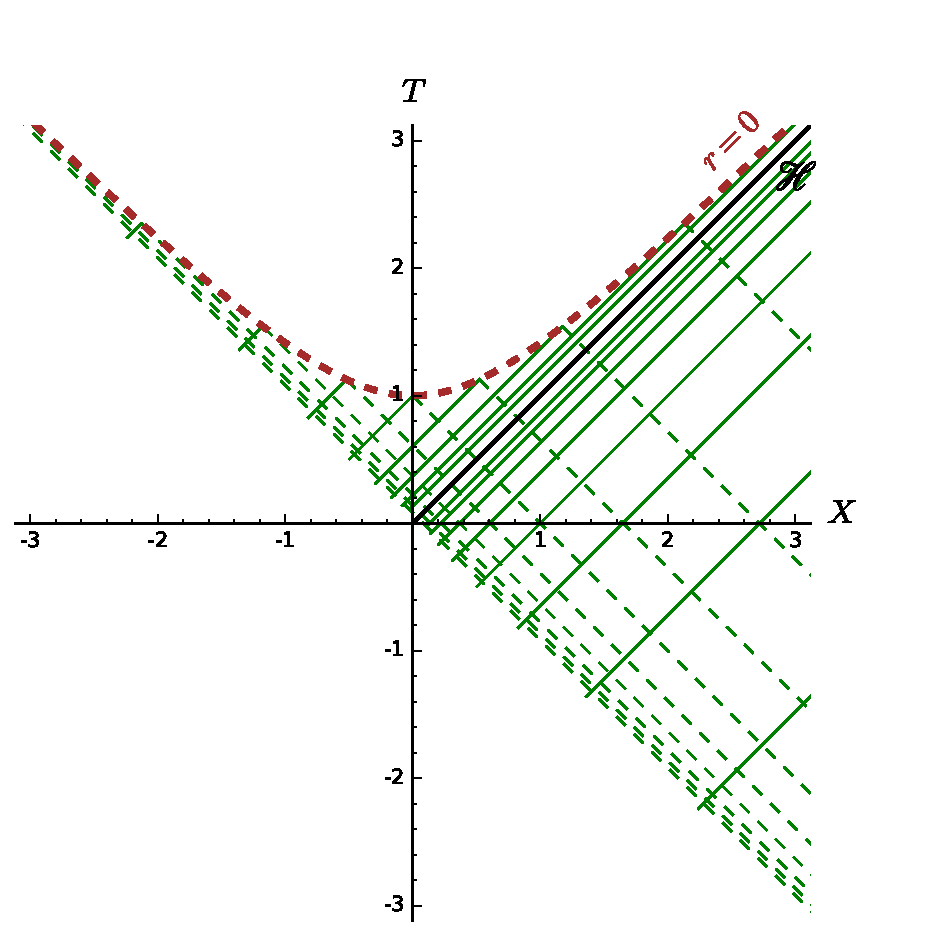
\includegraphics[width=0.6\textwidth]{sch_rad_null_geod_KS.pdf}}
\caption[]{\label{f:sch:rad_null_geod_KS} \footnotesize
Radial null geodesics in $\M_{\rm IEF} = \M_{\rm I}\cup\Hor\cup\M_{\rm II}$
depicted in terms of the Kruskal-Szekeres coordinates $(T,X)$: the solid
lines correspond to the outgoing family, with $u$ spanning $[-6m, 8m]$
(with steps $\delta u = 2m$), from the left to the right in $\M_{\rm II}$
and from the right to the left in $\M_{\rm I}$; the dashed lines
correspond to the ingoing family, with $v$ spanning $[-8m, 6m]$ (with steps $\delta v = 2m$)
from the left to the right.}
\end{figure}
In particular, the Schwarzschild horizon $\Hor$ is generated by the
outgoing radial null geodesics having $U=0$:
Eqs.~(\ref{e:sch:outgoing_null_geod_KS}) and (\ref{e:sch:X2mT2})
clearly imply $r=2m$ for $U=0$, i.e. $X=T$.
 The outgoing radial null geodesics not lying on $\Hor$ have an equation
in terms of the IEF coordinates given by
Eq.~(\ref{e:sch:outgoing_null_geod_EF}):
$\ti = r + 4 m \ln \left|r/2m- 1 \right| + u$,
where the constant $u$ is related to $U$ by
\begin{subequations}
\begin{align}
 & U = - \mathrm{e}^{-u/4m} \quad \mbox{on}\ \M_{\rm I} \\
 & U = 0 \quad \mbox{on}\ \Hor \\
 & U =  \mathrm{e}^{-u/4m} \quad \mbox{on}\ \M_{\rm II} .
\end{align}
\end{subequations}
These relations are easily established by combining
(\ref{e:sch:outgoing_null_geod_EF}) and (\ref{e:sch:KS_IEF}).


\begin{remark}
The relation $U = - \mathrm{e}^{-u/4m}$ introduced in Sec.~\ref{s:sch:KS_coord}
by Eq.~(\ref{e:sch:def_U_V}) is thus valid only in $\M_{\rm I}$. On the
contrary the relation $V = \mathrm{e}^{v/4m}$ is valid in all $\M_{\rm IEF}$.
\end{remark}

\section{Maximal extension} \label{s:sch:max_extens}

The spacetime $(\M_{\rm IEF}, \w{g})$ is not geodesically complete.
Indeed, let us consider the radial null geodesics discussed above.
We have seen in Sec.~\ref{s:sch:rad_null_geod} that $r$ is an affine parameter
along them, except for those that are null generators of $\Hor$
(the outgoing ones with $U=0$).
Now, for the ingoing radial null geodesics, $r$ is decreasing towards the
future and all of them terminate at $r=0$ (the left end-point of the dashed
lines in Fig.~\ref{f:sch:rad_null_geod_KS}).
They are thus incomplete geodesics. However, they cannot be extended to
negative values of the affine parameter $r$ by extending the spacetime
since $r=0$ marks a spacetime singularity (cf. Sec.~\ref{s:sch:singularities}).

On the other hand the outgoing radial null geodesics are limited by
the constraint $T+X > 0$, which corresponds to $r>2m$ in $\M_{\rm I}$, with $r$ increasing towards
the future, and to
$r<2m$ in $\M_{\rm II}$, with $r$ decreasing towards the future.
Thus all outgoing radial null geodesics terminate towards the past at the finite
value $2m$ of the affine parameter $r$
(the left end point of the solid lines in Fig.~\ref{f:sch:rad_null_geod_KS}) and are therefore incomplete geodesics.
However, contrary to ingoing radial null geodesics, they can be extended
since $r=2m$ does not mark any spacetime singularity.
More precisely, the limit at which outgoing radial null geodesics
terminate is $T=-X$, which by virtue of (\ref{e:sch:X2mT2}) yields $r=2m$.
This does not correspond to the Schwarzschild horizon $\Hor$, since for
the latter $T=X$, but rather to $\ti\rightarrow-\infty$,
as it is clear when comparing Fig.~\ref{f:sch:rad_null_geod_KS}
with Fig.~\ref{f:sch:IEF_KS}.

Another hint regarding the extendability of $(\M_{\rm IEF}, \w{g})$
is the fact that the Killing horizon $\Hor$ is non-degenerate, having
a non-zero surface gravity (cf. Sec.~\ref{s:neh:classif_KH}); the latter
has been computed in Example~\ref{x:def:Schw_hor3} of Chap.~\ref{s:def}:
$\kappa = 1/4m$. Now, we have seen in Sec.~\ref{s:sta:bifur_Killing_hor}
that non-degenerate Killing horizons have incomplete null generators
and, if they can be extended, they must be part of a
bifurcate Killing horizon. In the present case, the null generators of $\Hor$
are nothing but outgoing radial null geodesics. They are thus as incomplete
as those that admit $r$ as an affine parameter discussed above.

The possibility of spacetime extension beyond $\M_{\rm IEF}$ is clear
on the metric element (\ref{e:sch:metric_KS_TX_partial}): it is invariant by
the transformation
\be \label{e:sch:origin_reflection}
    \begin{array}{lccc}
    \Phi : & \R^2 & \longrightarrow & \R^2 \\
        & (T,X) & \longmapsto & (-T,-X) .
    \end{array}
\ee
Thus we may include
the part $T+X<0$ by adding a copy of $\M_{\rm IEF}$, symmetric to the
original one with respect to the ``origin'' $(T,X)=(0,0)$.
The whole spacetime manifold is then the following open subset of
$\R^2\times\mathbb{S}^2$:
\be \label{e:sch:def_M_extend}
    \M = \{ p \in \R^2\times\mathbb{S}^2, \quad X^2(p) - T^2(p) > - 1 \} ,
\ee
where $(T,X,\th,\ph)$ is the canonical coordinate system on $\R^2\times\mathbb{S}^2$,
called in this context
\defin{Kruskal-Szekeres coordinates}\index{Kruskal-Szekeres!coordinates}.
The metric $\w{g}$ on the whole $\M$ is then defined by (\ref{e:sch:metric_KS_TX_partial}):
\be \label{e:sch:metric_KS_TX}
   \encadre{
    \begin{array}{lcll}
    g_{\mu\nu} \, \D X^\mu \, \D X^\nu & = & 4m^2 \bigg\{ & \displaystyle
    \frac{4}{X^2-T^2 + \mathrm{e}^{F^{-1}(X^2-T^2)} }
    \left( - \D T^2 + \D X^2 \right) \\[2ex]
    & & & \displaystyle + \,   (F^{-1}(X^2-T^2))^2 \left( \D\th^2 + \sin^2\th\, \D\ph^2 \right)
    \bigg\} ,
    \end{array} }
\ee
where $F^{-1}$ is the inverse of the function $F(x) = \mathrm{e}^{x} (x-1)$,
which establishes a bijection from $(0,+\infty)$ to $(-1,+\infty)$.

\begin{figure}
\centerline{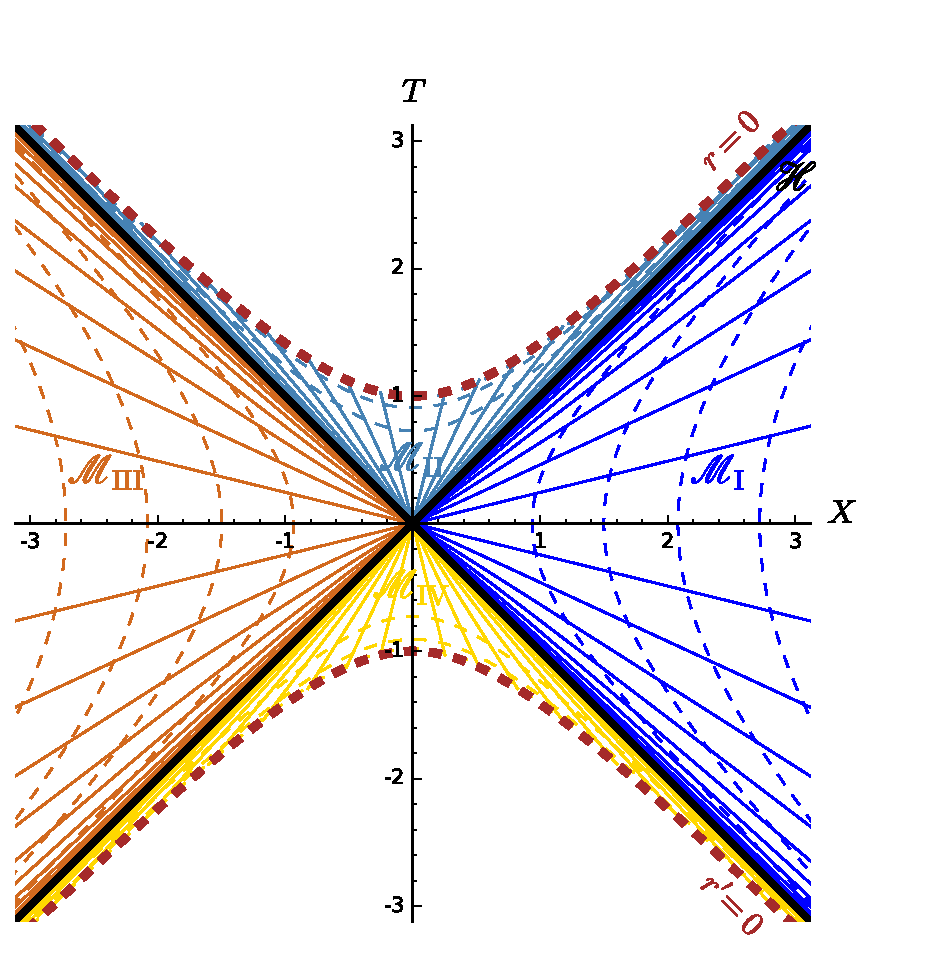
\includegraphics[width=0.6\textwidth]{sch_kruskal_diag.pdf}}
\caption[]{\label{f:sch:kruskal_diag} \footnotesize
Schwarzschild spacetime $\M$ depicted in terms of Kruskal-Szekeres coordinates $(T,X)$.
Each point in this diagram, including the one at $(T,X)=(0,0)$,
is actually a sphere $\SS^2$, spanned by the
coordinates $(\th,\ph)$.
Solid lines denote the hypersurfaces $t=\mathrm{const}$ in $\M_{\rm I}$ and
$\M_{\rm II}$ and the  hypersurfaces $t'=\mathrm{const}$ in $\M_{\rm III}$ and
$\M_{\rm IV}$, whiles dashed curves
denote the hypersurfaces $r=\mathrm{const}$ in $\M_{\rm I}$ and
$\M_{\rm II}$ and the  hypersurfaces $r'=\mathrm{const}$ in $\M_{\rm III}$ and
$\M_{\rm IV}$.
The bifurcate Killing horizon is marked by thick black lines, while the
singularities at $r=0$ and $r'=0$ are depicted by the heavy dashed brown curve.}
\end{figure}

Let us define the following open subsets of $\M$, which are respectively
the images of $\M_{\rm I}$ and $\M_{\rm II}$ by the reflection through the origin
(\ref{e:sch:origin_reflection}):
\begin{subequations}
\begin{align}
 & \M_{\rm III}: \quad X < 0 \quad\mbox{and}\quad X < T < -X \\
 & \M_{\rm IV}: \quad - \sqrt{X^2+1} < T < -|X| .
\end{align}
\end{subequations}
On $\M_{\rm III}\cup \M_{\rm IV}$, one may introduce coordinates
$(t',r',\th,\ph)$ of Schwarzschild-Droste type; they are related to
the Kruskal-Szekeres coordinates by formulas analoguous to
(\ref{e:sch:KS_SD_I}) and (\ref{e:sch:KS_SD_II}), simply changing $T$ to $-T$
and $X$ to $-X$:
\be \label{e:sch:KS_SD_III}
    \M_{\rm III}: \quad \encadre{ \left\{\begin{array}{l}
    T = - \mathrm{e}^{r'/4m} \sqrt{ \frac{r'}{2m} - 1 } \sinh\left( \frac{t'}{4m} \right)
\\[2ex]
    X = - \mathrm{e}^{r'/4m} \sqrt{ \frac{r'}{2m} - 1 } \cosh\left( \frac{t'}{4m} \right)
        \end{array}\right. }
    \iff
    \encadre{ \left\{\begin{array}{l}
    t' = 2 m \,  \ln \left( \frac{X+T}{X-T} \right) \\[2ex]
    r' = 2 m F^{-1}(X^2 - T^2) .
        \end{array}\right. }
\ee
\be \label{e:sch:KS_SD_IV}
    \M_{\rm IV}: \quad \encadre{ \left\{\begin{array}{l}
    T = - \mathrm{e}^{r'/4m} \sqrt{ 1 - \frac{r'}{2m} } \cosh\left( \frac{t'}{4m} \right)
\\[2ex]
    X = - \mathrm{e}^{r'/4m} \sqrt{ 1 - \frac{r'}{2m} } \sinh\left( \frac{t'}{4m} \right)
        \end{array}\right. }
    \iff
    \encadre{ \left\{\begin{array}{l}
    t' = 2 m \,  \ln \left( \frac{T+X}{T-X} \right) \\[2ex]
    r' = 2 m F^{-1}(X^2 - T^2) .
        \end{array}\right. }
\ee

The extended Schwarzschild spacetime $(\M,\w{g})$ is depicted in
Fig.~\ref{f:sch:kruskal_diag}, which is usually called a
\defin{Kruskal diagram}\index{Kruskal!diagram}.
There are two curvature singularities, which formally are not part of $\M$:
the hypersurfaces $r=0$ and $r'=0$.
As discussed in Sec.~\ref{s:sch:rad_null_geod_KS}, the radial null
geodesics appear as straight lines of slope $\pm 45^\circ$ ($+$ for the
outgoing family, and $-$ for the ingoing one).
As in $(\M_{\rm IEF},\w{g})$, they are still not complete but the only
locations where they terminate are the curvature singularities
at $r=0$ (future end point) and $r'=0$ (past end point). Therefore, they cannot
be extended further. For this reason, $(\M,\w{g})$ is called the
\defin{maximal extension}\index{maximal!extension}\index{extension!maximal --}
of Schwarzschild spacetime.



\section{Bifurcate Killing horizon}

As discussed in Sec.~\ref{s:sch:max_extens}, the Schwarzschild horizon
$\Hor$ is
a non-degenerate Killing horizon and therefore shall be part of
a bifurcate Killing horizon (cf. Sec.~\ref{s:sta:bifur_Killing_hor})
in the extended spacetime.
The bifurcate Killing horizon, $\hat{\Hor}$ say, is easily found by
considering the Killing vector field $\w{\xi}$ in the maximal extension
of Schwarzschild spacetime. The components of $\w{\xi}$ w.r.t. to the
Kruskal-Szekeres coordinates are obtained from the
property $\w{\xi} = \wpar_t$:
\[
    \xi^T = \der{T}{t}, \quad
    \xi^X = \der{X}{t}, \quad
    \xi^\th = \der{\th}{t} = 0, \quad
    \xi^\ph = \der{\ph}{t} = 0 .
\]
Given the coordinate transformation laws (\ref{e:sch:KS_SD_I})
and (\ref{e:sch:KS_SD_II}), we get in
$\M_{\rm I}$ and $\M_{\rm II}$:
\[
    \xi^T = \frac{1}{4m} \, X, \quad
    \xi^X = \frac{1}{4m} \, T , \quad
    \xi^\th = \xi^\ph = 0 .
\]
Hence in $\M_{\rm I}\cup\M_{\rm II}$,
\be \label{e:sch:xi_X_T}
    \encadre{ \w{\xi} = \frac{1}{4m} \left( X \, \wpar_T + T \, \wpar_X \right) }.
\ee
Now, this formula defines a smooth vector field in all $\M$.
Moreover, in $\M_{\rm III}\cup\M_{\rm IV}$, this vector coincides with
$\wpar_{t'}$ since $\xi^T = \dert{T}{t'}$ and $\xi^X = \dert{X}{t'}$,
with the partial derivatives with respect to $t'$ evaluated from
(\ref{e:sch:KS_SD_III})-(\ref{e:sch:KS_SD_IV}). Hence the vector field
$\w{\xi}$ defined by (\ref{e:sch:xi_X_T}) is a Killing vector field
of maximal extension $(\M,\w{g})$. This vector field is depicted in
Fig.~\ref{f:sch:xi_extend}.

\begin{figure}
\centerline{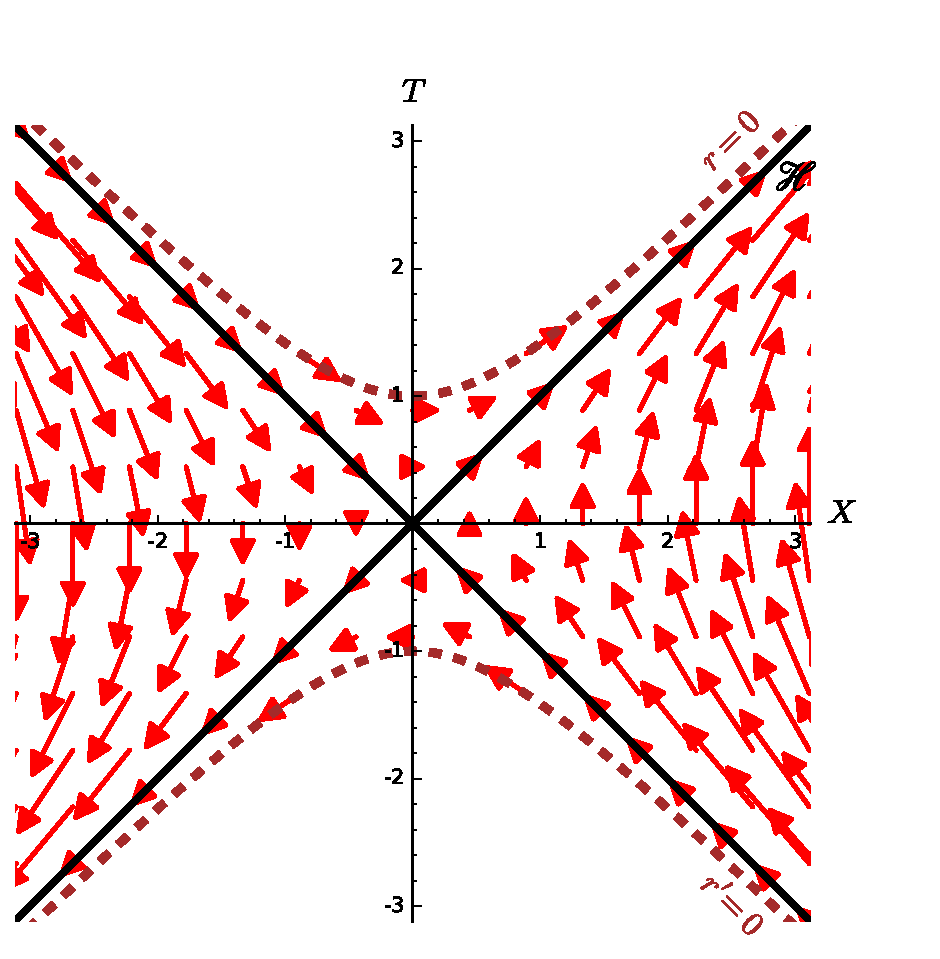
\includegraphics[width=0.6\textwidth]{sch_xi_extend.pdf}}
\caption[]{\label{f:sch:xi_extend} \footnotesize
Killing vector field $\w{\xi}$ on the extended Schwarzschild manifold.}
\end{figure}

The bifurcate Killing horizon with respect to $\w{\xi}$
that extends $\Hor$
is $\hat{\Hor} = \Hor_1 \cup \Hor_2 $, where
\begin{itemize}
\item $\Hor_1$ is the null hypersurface $T=X$;
\item $\Hor_2$ is the null hypersurface $T=-X$.
\end{itemize}
$\Hor$ is then the part of $\Hor_1$ defined by $X>0$.
The bifurcation surface is $\Sp = \Hor_1 \cap \Hor_2$, which
is the 2-surface defined by $T=0$ and $X=0$. It is a 2-sphere, since
any fixed value of the pair $(T,X)$ defines a 2-sphere, according to the
definition of $\M$ as a part of $\R^2\times\mathbb{S}^2$
[cf. Eq.~(\ref{e:sch:def_M_extend})]. Accordingly, $\Sp$ is called the
\defin{bifurcation sphere}\index{bifurcation!sphere}. It is located at the
center of Fig.~\ref{f:sch:xi_extend}.
The areal radius of $\Sp$ is found by setting
$\D T = 0$, $\D X = 0$ and $(T,X)=(0,0)$ in the line element
(\ref{e:sch:metric_KS_TX}):
\[
    r_{\Sp}^2 = 4m^2 (F^{-1}(0))^2.
\]
Since $F^{-1}(0)=1$, we get
\be
    \encadre{r_{\Sp} = 2 m } .
\ee
Moreover, setting $(T,X)=(0,0)$ in Eq.~(\ref{e:sch:xi_X_T}),
we recover the general property (\ref{e:sta:xi_S_zero}): the Killing
vector field vanishes identically at the bifurcation sphere:
\be
\left. \w{\xi} \right| _{\Sp} = 0 .
\ee


\section{Carter-Penrose diagram} \label{s:max:Carter-Penrose}

To have a compact representation of the maximal extension of Schwarzschild spacetime,
let us introduce ``finite-range'' coordinates $(\tilde{T},\tilde{X})$, which
are related to $(T,X)$ in exactly the same way as the coordinates $(\tau,\chi)$
are related to $(t,r)$ in the construction of the conformal completion of
Minkowski spacetime in
Sec.~\ref{s:glo:conf_Mink} [cf. Eq.~(\ref{e:glo:tau_chi_t_r})]
\be
    \left\{ \begin{array}{l}
    \tilde{T} = \arctan(T+X) + \arctan(T-X) \\
    \tilde{X} = \arctan(T+X) - \arctan(T-X)
    \end{array} \right.
    \iff
    \left\{ \begin{array}{l}
    \displaystyle T = \frac{\sin\tilde{T}}{\cos\tilde{T} + \cos\tilde{X}}\\[2ex]
    \displaystyle X = \frac{\sin\tilde{X}}{\cos\tilde{T} + \cos\tilde{X}} .
    \end{array} \right.
\ee
The range of $(\tilde{T},\tilde{X})$ is constrained by
\be
\tilde{X}\in(-\pi,\pi) \qquad\mbox{and}\qquad -\pi+|\tilde{X}| < \tilde{T} < \pi-|\tilde{X}| .
\ee
The maximal extension of Schwarzschild spacetime is depicted with respect
to the coordinates $(\tilde{T},\tilde{X})$ in Fig.~\ref{f:sch:sch_carter-penrose}.
Such a plot is called a \defin{Carter-Penrose diagram}\index{Carter-Penrose diagram}.
It is also called a \defin{conformal diagram}\index{conformal!diagram}.
As the Kruskal diagram (Fig.~\ref{f:sch:kruskal_diag}), it has the property
to display the null geodesics as straight lines with slope $\pm 45^\circ$.

\begin{figure}
\centerline{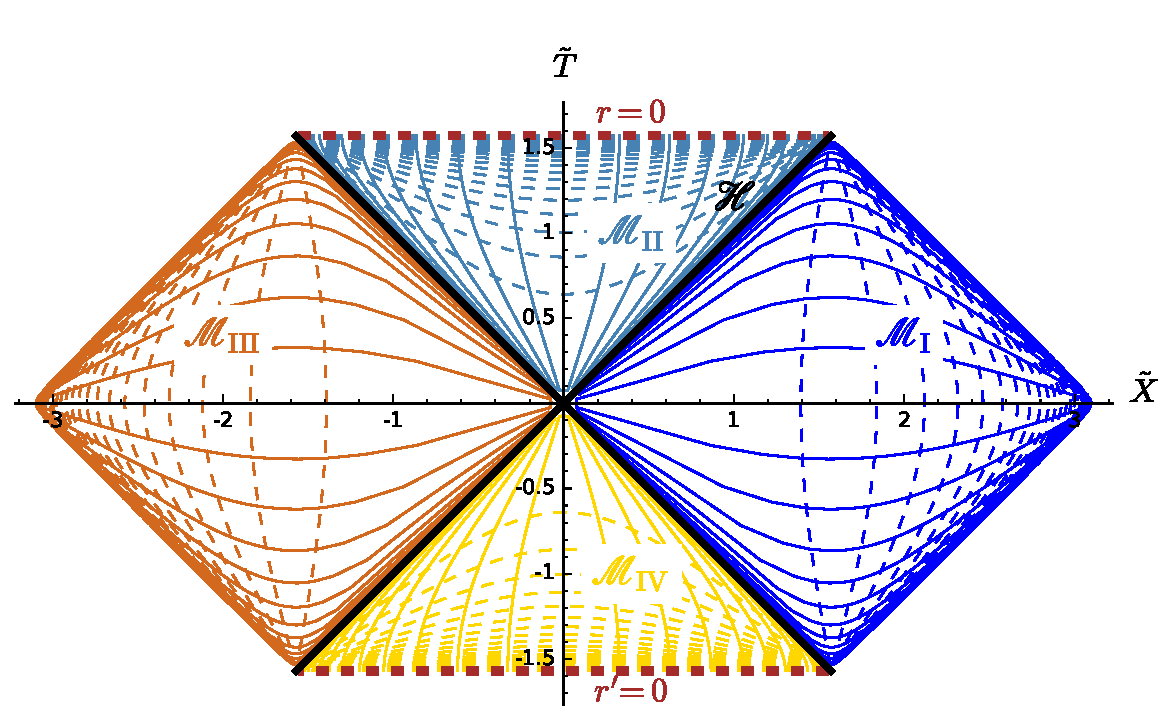
\includegraphics[width=0.9\textwidth]{sch_carter-penrose.pdf}}
\caption[]{\label{f:sch:sch_carter-penrose} \footnotesize
Carter-Penrose diagram of the Schwarzschild spacetime; the color code
is the same as in Fig.~\ref{f:sch:kruskal_diag}.
As the latter, this figure has been produced with
SageManifolds (cf. Appendix~\ref{s:sam}).}
\end{figure}

The Carter-Penrose diagram in Fig.~\ref{f:sch:sch_carter-penrose} can be compared with the conformal diagram
of Minkowski spacetime in Fig.~\ref{f:glo:conf_diag_Mink}.


\cite{HalacL14}

\section{Isotropic coordinates}


